\documentclass[10pt]{beamer}

\usetheme[progressbar=frametitle]{metropolis}
\usepackage{appendixnumberbeamer}

\usepackage{booktabs}

% For removing Figure 1 in figures
\usepackage{caption}

% For enumeration as words
\usepackage{blindtext}
\usepackage{enumerate}
\usepackage{geometry}

\usepackage{tikz}
\usepackage{xspace}


\title{Theory of Computation}
\subtitle{Tutorial - Regular Expressions}
\author{Cesare Spinoso-Di Piano}
\date{}

\begin{document}

\maketitle

\begin{frame}{Plan for today}
    \setbeamertemplate{section in toc}[sections numbered]
    \tableofcontents[hideallsubsections]
\end{frame}


\section{Regular expressions}
\begin{frame}{Regular expressions}
    \textbf{Definition.} Given an alphabet $\Sigma$, define a regular expression as follows:
    \begin{enumerate}[1.]
        \item $\emptyset, \lambda, a \in \Sigma$ are the \textbf{primitive} regular expressions.
        \item If $r_1$ and $r_2$ are regular expressions, then so are $r_1+r_2$, $r_1\cdot r_2$, $r_1^*$ and $(r_1)$.
        \item A string $s$ is a regular expression \textbf{if and only if} it can be obtained by applying operations in 2. to the primitive regular expressions in 1.
    \end{enumerate}
    \textbf{Examples.}
    \begin{itemize}
        \item \textbf{Example.} $\Sigma = \{a,b\}$, $(a + \lambda)\cdot(b\cdot a + \emptyset^*)$ is a valid regular expression.
        \item \textbf{Example.} $\Sigma = \{a,b\}$, $(a \textcolor{red}\cap \lambda) \textcolor{red}- (b^{\textcolor{red}R} \cdot \emptyset)$ is NOT a valid regular expression.
    \end{itemize}
\end{frame}

\begin{frame}{Regular expressions}
    \textbf{Definition.} Given the regular expressions $r$, $L(r)$ is the language \textbf{denoted by/represented by} the regular expression $r$ where
    \begin{itemize}
        \item[] $L(\emptyset) = \emptyset$, $L(\lambda) = \{\lambda\}$, $L(a) = \{a\}, a \in \Sigma$
        \item[] If $r_1, r_2$ are regular expressions
            \begin{itemize}
                \item[] $L(r_1+r_2) = L(r_1) \cup L(r_2)$
                \item[] $L(r_1r_2) = L(r_1)L(r_2)$
                \item[] $L(r_1^*) = (L(r_1))^*$
            \end{itemize}
    \end{itemize}

\end{frame}

\begin{frame}{Example}
    \textbf{Example.} Given the regular expressions $r = (a+bb)(ab)^*$, what is $L(r)$?
    \begin{align*}
        L(r) & = L((a+bb)(ab)^*)                                                                    \\
             & = L(a + bb) L((ab)^*)                                       & \text{Using 3.}        \\
             & = \Big{(} L(a) \cup L(bb)\Big{)} \Big{(} L(ab)\Big{)}^*     & \text{Using 2. and 4.} \\
             & = \Big{(} \{a\} \cup \{bb\}\Big{)} \Big{(} \{ab\} \Big{)}^* & \text{Using 1.}        \\
             & = \{a, bb\} \{ab\}^*                                                                 \\
             & = \{a(ab)^n: n \geq 0\} \cup \{bb(ab)^n : n \geq 0\}
    \end{align*}
\end{frame}

\begin{frame}[t]{Exercise}
    \textbf{Exercise.} Given the regular expressions $r = (0+01)(1+11)^*$, how many strings of length \textbf{3 or less} are there in $L(r)$?

\end{frame}

\begin{frame}[t]{Exercise}
    \textbf{Exercise.} What is the the shortest string in $L(((a+\lambda)\emptyset^* + b + \emptyset)^*) \cap L(a(ba)^*)$?
\end{frame}

\begin{frame}[t]{Exercise}
    \textbf{Exercise.} Write a regular expression $r$ such that $L(r) = \{w \in \{0,1\}^* : \text{w contains 101}\}$.
\end{frame}

\begin{frame}[t]{Exercise}
    \textbf{Exercise.} Write a regular expression $r$ such that $L(r) = \{w \in \{0,1\}^* : \text{w has even length}\}$.
\end{frame}

\begin{frame}[t]{Exercise}
    \textbf{Exercise.} Write a regular expression $r$ such that $L(r) = \{vwv: |v| = 2, v,w \in \{a,b\}^*\}$.
\end{frame}

\begin{frame}{Equivalent regular expressions}
    \textbf{Definition.} Two regular expressions $r_1,r_2$ are equivalent ($r_1 \equiv r_2$) if and only if $L(r_1) = L(r_2)$.\\ \bigskip
    \textbf{Example.} True or False. $(r+\emptyset)^*\lambda = r^*$.\\
    This is True since
    \begin{align*}
        L((r+\emptyset)^*\lambda) & = L((r+\emptyset)^*)L(\lambda)      \\
                                  & = (L(r+\emptyset))^*L(\lambda)      \\
                                  & = (L(r) \cup \emptyset)^*L(\lambda) \\
                                  & = (L(r))^*                          \\
                                  & = L(r^*)
    \end{align*}
    In general, regular expression ``arithmetic'' is avoided in favor of FA manipulations.
\end{frame}

\section{Regular Expressions to FAs}

\begin{frame}{Regular expressions to FAs}
    \textbf{Theorem.} Given a regular expression $r$, there exists an NFA $N$ such that $L(M) = L(r)$.

    \textbf{Corollary.} Given a regular expression $r$, there exists an FA $M$ such that $L(M) = L(r)$.
\end{frame}

\begin{frame}[t]{Example}
    \textbf{Example.} Given $r = ab^*aa+b(ba)^*$, find an FA $M$ such that $L(M) = L(r)$.
    \begin{enumerate}[1.]
        \item Split the language into components. Here we have $L(ab^*aa)$, $L(b)$, $L((ba)^*)$.
        \item Draw an FA for each regular language separately.

              An FA for $L(ab^*aa)$.
              \begin{center}
                  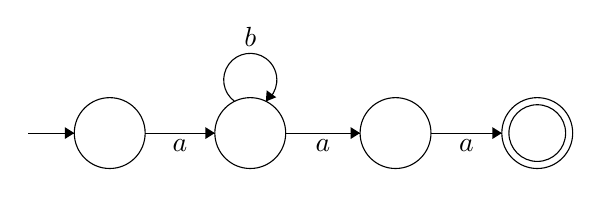
\begin{tikzpicture}[scale=0.15]
                      \tikzstyle{every node}+=[inner sep=0pt]
                      \draw [black] (12,-24.1) circle (3);
                      \draw [black] (23.9,-24.1) circle (3);
                      \draw [black] (36.2,-24.1) circle (3);
                      \draw [black] (48.2,-24.1) circle (3);
                      \draw [black] (48.2,-24.1) circle (2.4);
                      \draw [black] (15,-24.1) -- (20.9,-24.1);
                      \fill [black] (20.9,-24.1) -- (20.1,-23.6) -- (20.1,-24.6);
                      \draw (17.95,-24.6) node [below] {$a$};
                      \draw [black] (22.577,-21.42) arc (234:-54:2.25);
                      \draw (23.9,-16.85) node [above] {$b$};
                      \fill [black] (25.22,-21.42) -- (26.1,-21.07) -- (25.29,-20.48);
                      \draw [black] (26.9,-24.1) -- (33.2,-24.1);
                      \fill [black] (33.2,-24.1) -- (32.4,-23.6) -- (32.4,-24.6);
                      \draw (30.05,-24.6) node [below] {$a$};
                      \draw [black] (39.2,-24.1) -- (45.2,-24.1);
                      \fill [black] (45.2,-24.1) -- (44.4,-23.6) -- (44.4,-24.6);
                      \draw (42.2,-24.6) node [below] {$a$};
                      \draw [black] (5.1,-24.1) -- (9,-24.1);
                      \fill [black] (9,-24.1) -- (8.2,-23.6) -- (8.2,-24.6);
                  \end{tikzpicture}
              \end{center}
              An FA for $L(b)$.
              \begin{center}
                  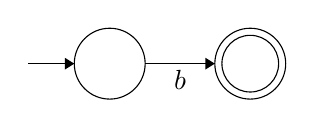
\begin{tikzpicture}[scale=0.15]
                      \tikzstyle{every node}+=[inner sep=0pt]
                      \draw [black] (12,-24.1) circle (3);
                      \draw [black] (23.9,-24.1) circle (3);
                      \draw [black] (23.9,-24.1) circle (2.4);
                      \draw [black] (15,-24.1) -- (20.9,-24.1);
                      \fill [black] (20.9,-24.1) -- (20.1,-23.6) -- (20.1,-24.6);
                      \draw (17.95,-24.6) node [below] {$b$};
                      \draw [black] (5.1,-24.1) -- (9,-24.1);
                      \fill [black] (9,-24.1) -- (8.2,-23.6) -- (8.2,-24.6);
                  \end{tikzpicture}
              \end{center}
    \end{enumerate}

\end{frame}

\begin{frame}[t]{Example}
    An FA for $L((ba)^*)$.
    \begin{center}
        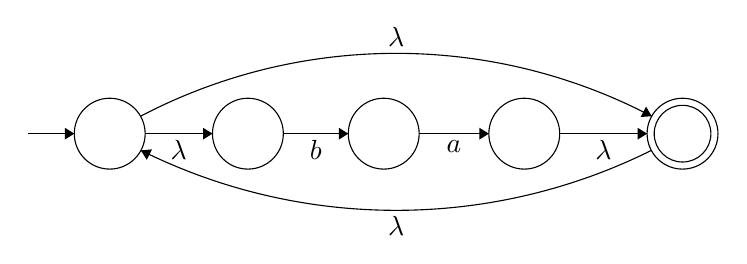
\begin{tikzpicture}[scale=0.15]
            \tikzstyle{every node}+=[inner sep=0pt]
            \draw [black] (10.5,-25) circle (3);
            \draw [black] (22.2,-25) circle (3);
            \draw [black] (45.6,-25) circle (3);
            \draw [black] (59,-25) circle (3);
            \draw [black] (59,-25) circle (2.4);
            \draw [black] (33.7,-25) circle (3);
            \draw [black] (3.6,-25) -- (7.5,-25);
            \fill [black] (7.5,-25) -- (6.7,-24.5) -- (6.7,-25.5);
            \draw [black] (13.5,-25) -- (19.2,-25);
            \fill [black] (19.2,-25) -- (18.4,-24.5) -- (18.4,-25.5);
            \draw (16.35,-25.5) node [below] {$\lambda$};
            \draw [black] (48.6,-25) -- (56,-25);
            \fill [black] (56,-25) -- (55.2,-24.5) -- (55.2,-25.5);
            \draw (52.3,-25.5) node [below] {$\lambda$};
            \draw [black] (25.2,-25) -- (30.7,-25);
            \fill [black] (30.7,-25) -- (29.9,-24.5) -- (29.9,-25.5);
            \draw (27.95,-25.5) node [below] {$b$};
            \draw [black] (36.7,-25) -- (42.6,-25);
            \fill [black] (42.6,-25) -- (41.8,-24.5) -- (41.8,-25.5);
            \draw (39.65,-25.5) node [below] {$a$};
            \draw [black] (13.111,-23.523) arc (117.65318:62.34682:46.625);
            \fill [black] (56.39,-23.52) -- (55.91,-22.71) -- (55.45,-23.59);
            \draw (34.75,-17.7) node [above] {$\lambda$};
            \draw [black] (56.357,-26.418) arc (-63.56281:-116.43719:48.531);
            \fill [black] (13.14,-26.42) -- (13.64,-27.22) -- (14.08,-26.33);
            \draw (34.75,-31.99) node [below] {$\lambda$};
        \end{tikzpicture}
    \end{center}
    An FA for $L(b(ba)^*)$.
    \begin{center}
        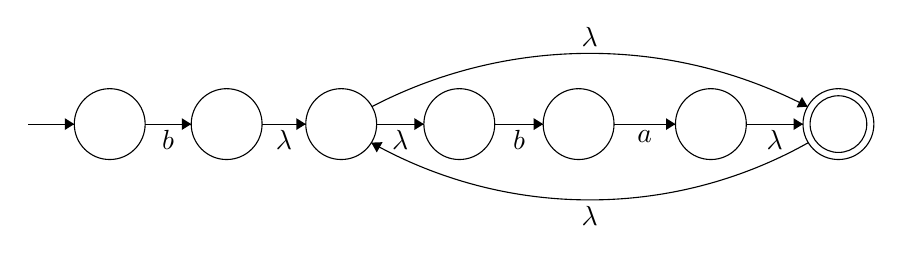
\begin{tikzpicture}[scale=0.15]
            \tikzstyle{every node}+=[inner sep=0pt]
            \draw [black] (9.5,-25.3) circle (3);
            \draw [black] (19.4,-25.3) circle (3);
            \draw [black] (29.1,-25.3) circle (3);
            \draw [black] (39.1,-25.3) circle (3);
            \draw [black] (49.2,-25.3) circle (3);
            \draw [black] (60.4,-25.3) circle (3);
            \draw [black] (71.2,-25.3) circle (3);
            \draw [black] (71.2,-25.3) circle (2.4);
            \draw [black] (2.6,-25.3) -- (6.5,-25.3);
            \fill [black] (6.5,-25.3) -- (5.7,-24.8) -- (5.7,-25.8);
            \draw [black] (12.5,-25.3) -- (16.4,-25.3);
            \fill [black] (16.4,-25.3) -- (15.6,-24.8) -- (15.6,-25.8);
            \draw (14.45,-25.8) node [below] {$b$};
            \draw [black] (22.4,-25.3) -- (26.1,-25.3);
            \fill [black] (26.1,-25.3) -- (25.3,-24.8) -- (25.3,-25.8);
            \draw (24.25,-25.8) node [below] {$\lambda$};
            \draw [black] (32.1,-25.3) -- (36.1,-25.3);
            \fill [black] (36.1,-25.3) -- (35.3,-24.8) -- (35.3,-25.8);
            \draw (34.1,-25.8) node [below] {$\lambda$};
            \draw [black] (42.1,-25.3) -- (46.2,-25.3);
            \fill [black] (46.2,-25.3) -- (45.4,-24.8) -- (45.4,-25.8);
            \draw (44.15,-25.8) node [below] {$b$};
            \draw [black] (52.2,-25.3) -- (57.4,-25.3);
            \fill [black] (57.4,-25.3) -- (56.6,-24.8) -- (56.6,-25.8);
            \draw (54.8,-25.8) node [below] {$a$};
            \draw [black] (63.4,-25.3) -- (68.2,-25.3);
            \fill [black] (68.2,-25.3) -- (67.4,-24.8) -- (67.4,-25.8);
            \draw (65.8,-25.8) node [below] {$\lambda$};
            \draw [black] (68.647,-26.873) arc (-60.63664:-119.36336:37.722);
            \fill [black] (31.65,-26.87) -- (32.11,-27.7) -- (32.6,-26.83);
            \draw (50.15,-32.22) node [below] {$\lambda$};
            \draw [black] (31.707,-23.817) arc (117.47276:62.52724:39.978);
            \fill [black] (68.59,-23.82) -- (68.11,-23) -- (67.65,-23.89);
            \draw (50.15,-18.81) node [above] {$\lambda$};
        \end{tikzpicture}
    \end{center}
\end{frame}

\begin{frame}[t]{Example}
    Combining all these machines together.
    \begin{center}
        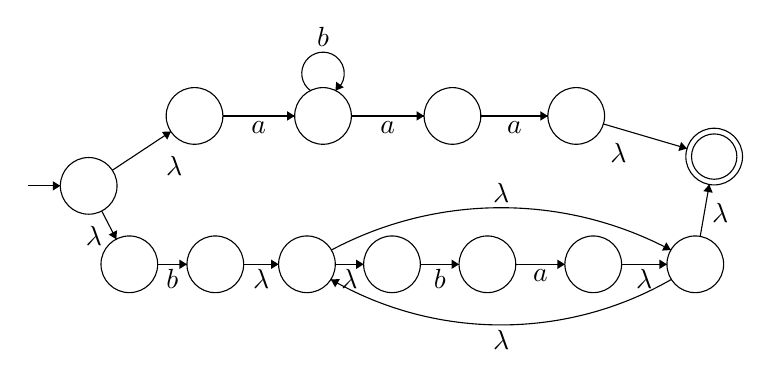
\begin{tikzpicture}[scale=0.12]
            \tikzstyle{every node}+=[inner sep=0pt]
            \draw [black] (11.3,-25.3) circle (3);
            \draw [black] (20.4,-25.3) circle (3);
            \draw [black] (30.1,-25.3) circle (3);
            \draw [black] (39.1,-25.3) circle (3);
            \draw [black] (49.2,-25.3) circle (3);
            \draw [black] (60.4,-25.3) circle (3);
            \draw [black] (71.2,-25.3) circle (3);
            \draw [black] (18.2,-9.6) circle (3);
            \draw [black] (31.8,-9.6) circle (3);
            \draw [black] (45.5,-9.6) circle (3);
            \draw [black] (58.6,-9.6) circle (3);
            \draw [black] (73.2,-13.9) circle (3);
            \draw [black] (73.2,-13.9) circle (2.4);
            \draw [black] (7,-17) circle (3);
            \draw [black] (14.3,-25.3) -- (17.4,-25.3);
            \fill [black] (17.4,-25.3) -- (16.6,-24.8) -- (16.6,-25.8);
            \draw (15.85,-25.8) node [below] {$b$};
            \draw [black] (23.4,-25.3) -- (27.1,-25.3);
            \fill [black] (27.1,-25.3) -- (26.3,-24.8) -- (26.3,-25.8);
            \draw (25.25,-25.8) node [below] {$\lambda$};
            \draw [black] (33.1,-25.3) -- (36.1,-25.3);
            \fill [black] (36.1,-25.3) -- (35.3,-24.8) -- (35.3,-25.8);
            \draw (34.6,-25.8) node [below] {$\lambda$};
            \draw [black] (42.1,-25.3) -- (46.2,-25.3);
            \fill [black] (46.2,-25.3) -- (45.4,-24.8) -- (45.4,-25.8);
            \draw (44.15,-25.8) node [below] {$b$};
            \draw [black] (52.2,-25.3) -- (57.4,-25.3);
            \fill [black] (57.4,-25.3) -- (56.6,-24.8) -- (56.6,-25.8);
            \draw (54.8,-25.8) node [below] {$a$};
            \draw [black] (63.4,-25.3) -- (68.2,-25.3);
            \fill [black] (68.2,-25.3) -- (67.4,-24.8) -- (67.4,-25.8);
            \draw (65.8,-25.8) node [below] {$\lambda$};
            \draw [black] (68.665,-26.903) arc (-60.06518:-119.93482:36.102);
            \fill [black] (32.63,-26.9) -- (33.08,-27.74) -- (33.58,-26.87);
            \draw (50.65,-32.22) node [below] {$\lambda$};
            \draw [black] (32.691,-23.789) arc (118.00545:61.99455:38.247);
            \fill [black] (68.61,-23.79) -- (68.14,-22.97) -- (67.67,-23.85);
            \draw (50.65,-18.81) node [above] {$\lambda$};
            \draw [black] (71.72,-22.35) -- (72.68,-16.85);
            \fill [black] (72.68,-16.85) -- (72.05,-17.56) -- (73.04,-17.73);
            \draw (72.92,-19.85) node [right] {$\lambda$};
            \draw [black] (61.48,-10.45) -- (70.32,-13.05);
            \fill [black] (70.32,-13.05) -- (69.7,-12.35) -- (69.41,-13.31);
            \draw (63.06,-12.43) node [below] {$\lambda$};
            \draw [black] (48.5,-9.6) -- (55.6,-9.6);
            \fill [black] (55.6,-9.6) -- (54.8,-9.1) -- (54.8,-10.1);
            \draw (52.05,-10.1) node [below] {$a$};
            \draw [black] (34.8,-9.6) -- (42.5,-9.6);
            \fill [black] (42.5,-9.6) -- (41.7,-9.1) -- (41.7,-10.1);
            \draw (38.65,-10.1) node [below] {$a$};
            \draw [black] (21.2,-9.6) -- (28.8,-9.6);
            \fill [black] (28.8,-9.6) -- (28,-9.1) -- (28,-10.1);
            \draw (25,-10.1) node [below] {$a$};
            \draw [black] (30.477,-6.92) arc (234:-54:2.25);
            \draw (31.8,-2.35) node [above] {$b$};
            \fill [black] (33.12,-6.92) -- (34,-6.57) -- (33.19,-5.98);
            \draw [black] (9.5,-15.35) -- (15.7,-11.25);
            \fill [black] (15.7,-11.25) -- (14.75,-11.28) -- (15.31,-12.11);
            \draw (16.04,-13.8) node [below] {$\lambda$};
            \draw [black] (8.38,-19.66) -- (9.92,-22.64);
            \fill [black] (9.92,-22.64) -- (10,-21.7) -- (9.11,-22.16);
            \draw (8.46,-22.29) node [left] {$\lambda$};
            \draw [black] (0.6,-17) -- (4,-17);
            \fill [black] (4,-17) -- (3.2,-16.5) -- (3.2,-17.5);
        \end{tikzpicture}
    \end{center}
\end{frame}

\begin{frame}[t]{Exercise}
    \textbf{Exercise.} Create an NFA and a DFA that accept $L((abb)^*+(a^*bb^*))$.
\end{frame}

\section{FAs to Regular Expressions}

\begin{frame}{Generalized Transition Graph}
    \textbf{Theorem.} Given a finite automaton $M$, there exists a regular expressions $r$ such that $L(r) = L(M)$.

    How can we convert a finite automata to a regular expression? \underline{Generalized Transition Graphs.}

    \textbf{Definition.} A generalized transition graph is a transition graph whose edges are labeled with regular expressions. Therefore, the transition $\delta'(q, r)$ executes if the GTG reads any string that belongs to $L(r)$.

    \textbf{Example.} The following GTG is of an FA that accepts $L(a^*(ba+a)(b+\lambda)a^*)$.
    \begin{center}
        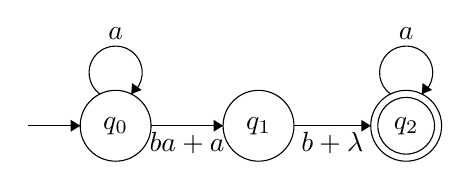
\begin{tikzpicture}[scale=0.15]
            \tikzstyle{every node}+=[inner sep=0pt]
            \draw [black] (16.2,-26.5) circle (3);
            \draw (16.2,-26.5) node {$q_0$};
            \draw [black] (28.3,-26.5) circle (3);
            \draw (28.3,-26.5) node {$q_1$};
            \draw [black] (40.8,-26.5) circle (3);
            \draw (40.8,-26.5) node {$q_2$};
            \draw [black] (40.8,-26.5) circle (2.4);
            \draw [black] (8.8,-26.5) -- (13.2,-26.5);
            \fill [black] (13.2,-26.5) -- (12.4,-26) -- (12.4,-27);
            \draw [black] (19.2,-26.5) -- (25.3,-26.5);
            \fill [black] (25.3,-26.5) -- (24.5,-26) -- (24.5,-27);
            \draw (22.25,-27) node [below] {$ba+a$};
            \draw [black] (14.877,-23.82) arc (234:-54:2.25);
            \draw (16.2,-19.25) node [above] {$a$};
            \fill [black] (17.52,-23.82) -- (18.4,-23.47) -- (17.59,-22.88);
            \draw [black] (31.3,-26.5) -- (37.8,-26.5);
            \fill [black] (37.8,-26.5) -- (37,-26) -- (37,-27);
            \draw (34.55,-27) node [below] {$b+\lambda$};
            \draw [black] (39.477,-23.82) arc (234:-54:2.25);
            \draw (40.8,-19.25) node [above] {$a$};
            \fill [black] (42.12,-23.82) -- (43,-23.47) -- (42.19,-22.88);
        \end{tikzpicture}
    \end{center}
\end{frame}

\begin{frame}{FA to RegExp}
    \textbf{How can we convert a finite automata to a regular expression using GTGs?}
    \begin{enumerate}[1.]
        \item Convert the FA to an NFA with a single final state (which should be distinct from $q_0$).
        \item Convert the FA to a GTG.
        \item Remove each intermediate state while preserving its role in the GTG.
        \item Repeat until only the initial and final states are left.
    \end{enumerate}

    The resulting GTG should have the following form.

    \begin{center}
        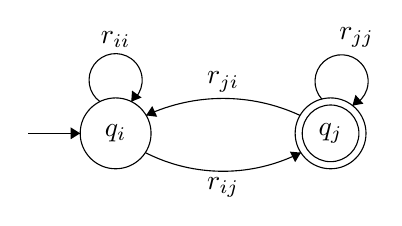
\begin{tikzpicture}[scale=0.15]
            \tikzstyle{every node}+=[inner sep=0pt]
            \draw [black] (10.3,-23) circle (3);
            \draw (10.3,-23) node {$q_i$};
            \draw [black] (28.5,-23) circle (3);
            \draw (28.5,-23) node {$q_j$};
            \draw [black] (28.5,-23) circle (2.4);
            \draw [black] (2.9,-23) -- (7.3,-23);
            \fill [black] (7.3,-23) -- (6.5,-22.5) -- (6.5,-23.5);
            \draw [black] (27.761,-20.105) arc (222.05768:-65.94232:2.25);
            \draw (30.7,-15.78) node [above] {$r_{jj}$};
            \fill [black] (30.35,-20.65) -- (31.28,-20.49) -- (30.61,-19.74);
            \draw [black] (25.987,-24.629) arc (-62.97266:-117.02734:14.496);
            \fill [black] (25.99,-24.63) -- (25.05,-24.55) -- (25.5,-25.44);
            \draw (19.4,-26.71) node [below] {$r_{ij}$};
            \draw [black] (12.882,-21.482) arc (114.89861:65.10139:15.481);
            \fill [black] (12.88,-21.48) -- (13.82,-21.6) -- (13.4,-20.69);
            \draw (19.4,-19.54) node [above] {$r_{ji}$};
            \draw [black] (8.977,-20.32) arc (234:-54:2.25);
            \draw (10.3,-15.75) node [above] {$r_{ii}$};
            \fill [black] (11.62,-20.32) -- (12.5,-19.97) -- (11.69,-19.38);
        \end{tikzpicture}
    \end{center}
    Then we see that this GTG reduces to the regular expression: $r = {{r_{ii}}^*}r_{ij}(r_{jj} + r_{ji}{{r_{ii}}^*}r_{ij})^*$

\end{frame}


\begin{frame}{FA to RegExp}

    A more detailed explanation of the algorithm.

    \begin{enumerate}[1.]
        \item Convert the FA to an NFA with a single final state (which should be distinct from $q_0$).
        \item Convert the NFA into a generalized transition graph. Let $r_{ij}$ stand for the label (a regular expression) of the edge from $q_i$ to $q_j$.
        \item If the GTG only has the initial state $q_i$ and final state $q_j$, compute the final regular expression $r = {{r_{ii}}^*}r_{ij}(r_{jj} + r_{ji}{{r_{ii}}^*}r_{ij})^*$.
              \begin{center}
                  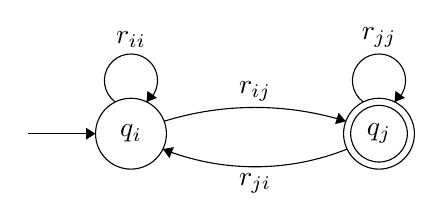
\begin{tikzpicture}[scale=0.15]
                      \tikzstyle{every node}+=[inner sep=0pt]
                      \draw [black] (15.4,-24.8) circle (3);
                      \draw (15.4,-24.8) node {$q_i$};
                      \draw [black] (36.4,-24.8) circle (3);
                      \draw (36.4,-24.8) node {$q_j$};
                      \draw [black] (36.4,-24.8) circle (2.4);
                      \draw [black] (6.7,-24.8) -- (12.4,-24.8);
                      \fill [black] (12.4,-24.8) -- (11.6,-24.3) -- (11.6,-25.3);
                      \draw [black] (14.077,-22.12) arc (234:-54:2.25);
                      \draw (15.4,-17.55) node [above] {$r_{ii}$};
                      \fill [black] (16.72,-22.12) -- (17.6,-21.77) -- (16.79,-21.18);
                      \draw [black] (18.207,-23.745) arc (107.2762:72.7238:25.905);
                      \fill [black] (33.59,-23.75) -- (32.98,-23.03) -- (32.68,-23.99);
                      \draw (25.9,-22.08) node [above] {$r_{ij}$};
                      \draw [black] (33.701,-26.105) arc (-68.27195:-111.72805:21.074);
                      \fill [black] (18.1,-26.1) -- (18.66,-26.87) -- (19.03,-25.94);
                      \draw (25.9,-28.1) node [below] {$r_{ji}$};
                      \draw [black] (35.077,-22.12) arc (234:-54:2.25);
                      \draw (36.4,-17.55) node [above] {$r_{jj}$};
                      \fill [black] (37.72,-22.12) -- (38.6,-21.77) -- (37.79,-21.18);
                  \end{tikzpicture}
              \end{center}
    \end{enumerate}
\end{frame}

\begin{frame}{FA to RegExp}
    \begin{enumerate}[4.]
        \item If the GTG has three states, the initial $q_i$ state, the final state $q_j$ and third state $q_k$. Introduce new edges, labeled $r_{pq} + r_{pk}{{r_{kk}}^*}r_{kq}$, for $p = i, j, q = i, j$. When this is done, remove $q_k$ and its associated edges.\\
              \begin{columns}
                  \column{0.5\textwidth}
                  \begin{center}
                      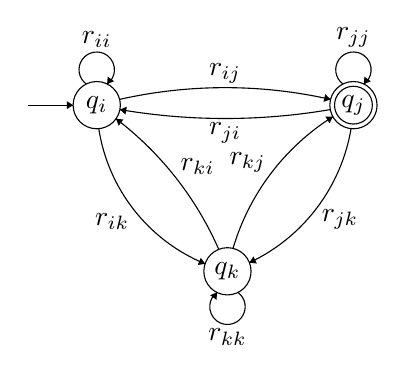
\begin{tikzpicture}[scale=0.1]
                          \tikzstyle{every node}+=[inner sep=0pt]
                          \draw [black] (15.4,-24.8) circle (3);
                          \draw (15.4,-24.8) node {$q_i$};
                          \draw [black] (48,-24.8) circle (3);
                          \draw (48,-24.8) node {$q_j$};
                          \draw [black] (48,-24.8) circle (2.4);
                          \draw [black] (32,-45.9) circle (3);
                          \draw (32,-45.9) node {$q_k$};
                          \draw [black] (6.7,-24.8) -- (12.4,-24.8);
                          \fill [black] (12.4,-24.8) -- (11.6,-24.3) -- (11.6,-25.3);
                          \draw [black] (14.077,-22.12) arc (234:-54:2.25);
                          \draw (15.4,-17.55) node [above] {$r_{ii}$};
                          \fill [black] (16.72,-22.12) -- (17.6,-21.77) -- (16.79,-21.18);
                          \draw [black] (18.309,-24.068) arc (102.7139:77.2861:60.845);
                          \fill [black] (45.09,-24.07) -- (44.42,-23.4) -- (44.2,-24.38);
                          \draw (31.7,-22.08) node [above] {$r_{ij}$};
                          \draw [black] (45.053,-25.362) arc (-80.29554:-99.70446:79.216);
                          \fill [black] (18.35,-25.36) -- (19.05,-25.99) -- (19.22,-25);
                          \draw (31.7,-27) node [below] {$r_{ji}$};
                          \draw [black] (46.677,-22.12) arc (234:-54:2.25);
                          \draw (48,-17.55) node [above] {$r_{jj}$};
                          \fill [black] (49.32,-22.12) -- (50.2,-21.77) -- (49.39,-21.18);
                          \draw [black] (29.158,-44.947) arc (-112.40505:-171.20858:22.238);
                          \fill [black] (29.16,-44.95) -- (28.61,-44.18) -- (28.23,-45.1);
                          \draw (19.59,-39.55) node [left] {$r_{ik}$};
                          \draw [black] (17.85,-26.531) arc (52.71749:23.66888:42.062);
                          \fill [black] (17.85,-26.53) -- (18.18,-27.41) -- (18.79,-26.62);
                          \draw (25.99,-32.57) node [right] {$r_{ki}$};
                          \draw [black] (32.706,-42.985) arc (163.50026:122.15411:29.718);
                          \fill [black] (45.38,-26.27) -- (44.44,-26.27) -- (44.97,-27.11);
                          \draw (36.95,-32.07) node [left] {$r_{kj}$};
                          \draw [black] (47.696,-27.782) arc (-9.54335:-64.80229:23.03);
                          \fill [black] (34.79,-44.8) -- (35.73,-44.91) -- (35.3,-44.01);
                          \draw (43.91,-39.28) node [right] {$r_{jk}$};
                          \draw [black] (33.323,-48.58) arc (54:-234:2.25);
                          \draw (32,-53.15) node [below] {$r_{kk}$};
                          \fill [black] (30.68,-48.58) -- (29.8,-48.93) -- (30.61,-49.52);
                      \end{tikzpicture}
                  \end{center}
                  \column{0.5\textwidth}
                  \begin{center}
                      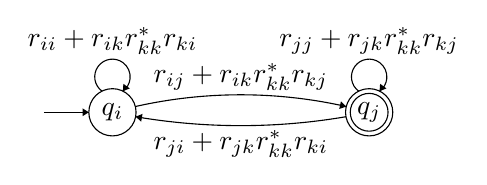
\begin{tikzpicture}[scale=0.1]
                          \tikzstyle{every node}+=[inner sep=0pt]
                          \draw [black] (15.4,-24.8) circle (3);
                          \draw (15.4,-24.8) node {$q_i$};
                          \draw [black] (48,-24.8) circle (3);
                          \draw (48,-24.8) node {$q_j$};
                          \draw [black] (48,-24.8) circle (2.4);
                          \draw [black] (6.7,-24.8) -- (12.4,-24.8);
                          \fill [black] (12.4,-24.8) -- (11.6,-24.3) -- (11.6,-25.3);
                          \draw [black] (14.077,-22.12) arc (234:-54:2.25);
                          \draw (15.4,-17.55) node [above] {$r_{ii}+r_{ik}r_{kk}^*r_{ki}$};
                          \fill [black] (16.72,-22.12) -- (17.6,-21.77) -- (16.79,-21.18);
                          \draw [black] (18.309,-24.068) arc (102.7139:77.2861:60.845);
                          \fill [black] (45.09,-24.07) -- (44.42,-23.4) -- (44.2,-24.38);
                          \draw (31.7,-22.08) node [above] {$r_{ij}+r_{ik}r_{kk}^*r_{kj}$};
                          \draw [black] (45.053,-25.362) arc (-80.29554:-99.70446:79.216);
                          \fill [black] (18.35,-25.36) -- (19.05,-25.99) -- (19.22,-25);
                          \draw (31.7,-27) node [below] {$r_{ji}+r_{jk}r_{kk}^*r_{ki}$};
                          \draw [black] (46.677,-22.12) arc (234:-54:2.25);
                          \draw (48,-17.55) node [above] {$r_{jj}+r_{jk}r_{kk}^*r_{kj}$};
                          \fill [black] (49.32,-22.12) -- (50.2,-21.77) -- (49.39,-21.18);
                      \end{tikzpicture}
                  \end{center}
              \end{columns}
    \end{enumerate}
\end{frame}

\begin{frame}[t]{FA to RegExp}
    \begin{itemize}
        \item[] 5. If the GTG has more than three states, pick a state $q_k$, apply the equation in step 4 for all pairs of states $(q_i,q_j)$, $i\neq k, j\neq k$.
        \item[] 6. Repeat step 2 to 4 until the GTG has only an initial and final state and then apply $r = {{r_{ii}}^*}r_{ij}(r_{jj} + r_{ji}{{r_{ii}}^*}r_{ij})^*$.
    \end{itemize}
\end{frame}

\begin{frame}{Example}
    \textbf{Example.} Find a regular expression that \textbf{denotes} the language \textbf{accepted} by the following NFA.\par
    \begin{center}
        \begin{tikzpicture}[scale=0.2]
            \tikzstyle{every node}+=[inner sep=0pt]
            \draw [black] (17.6,-26.1) circle (3);
            \draw (17.6,-26.1) node {$1$};
            \draw [black] (36.7,-26.1) circle (3);
            \draw (36.7,-26.1) node {$2$};
            \draw [black] (26.7,-11.7) circle (3);
            \draw (26.7,-11.7) node {$4$};
            \draw [black] (54.3,-26.1) circle (3);
            \draw (54.3,-26.1) node {$3$};
            \draw [black] (54.3,-26.1) circle (2.4);
            \draw [black] (9.8,-26.1) -- (14.6,-26.1);
            \fill [black] (14.6,-26.1) -- (13.8,-25.6) -- (13.8,-26.6);
            \draw [black] (19.2,-23.56) -- (25.1,-14.24);
            \fill [black] (25.1,-14.24) -- (24.25,-14.65) -- (25.09,-15.18);
            \draw (22.78,-20.2) node [right] {$b$};
            \draw [black] (28.41,-14.16) -- (34.99,-23.64);
            \fill [black] (34.99,-23.64) -- (34.94,-22.69) -- (34.12,-23.26);
            \draw (31.1,-20.26) node [left] {$b$};
            \draw [black] (20.6,-26.1) -- (33.7,-26.1);
            \fill [black] (33.7,-26.1) -- (32.9,-25.6) -- (32.9,-26.6);
            \draw (27.15,-26.6) node [below] {$a,b$};
            \draw [black] (38.023,-28.78) arc (54:-234:2.25);
            \draw (36.7,-33.35) node [below] {$b$};
            \fill [black] (35.38,-28.78) -- (34.5,-29.13) -- (35.31,-29.72);
            \draw [black] (39.7,-26.1) -- (51.3,-26.1);
            \fill [black] (51.3,-26.1) -- (50.5,-25.6) -- (50.5,-26.6);
            \draw (45.5,-26.6) node [below] {$a$};
        \end{tikzpicture}
    \end{center}

\end{frame}


\begin{frame}{Example}
    The equivalent GTG.

    \begin{center}
        \begin{tikzpicture}[scale=0.2]
            \tikzstyle{every node}+=[inner sep=0pt]
            \draw [black] (17.6,-26.1) circle (3);
            \draw (17.6,-26.1) node {$1$};
            \draw [black] (36.7,-26.1) circle (3);
            \draw (36.7,-26.1) node {$2$};
            \draw [black] (26.7,-11.7) circle (3);
            \draw (26.7,-11.7) node {$4$};
            \draw [black] (54.3,-26.1) circle (3);
            \draw (54.3,-26.1) node {$3$};
            \draw [black] (54.3,-26.1) circle (2.4);
            \draw [black] (9.8,-26.1) -- (14.6,-26.1);
            \fill [black] (14.6,-26.1) -- (13.8,-25.6) -- (13.8,-26.6);
            \draw [black] (19.2,-23.56) -- (25.1,-14.24);
            \fill [black] (25.1,-14.24) -- (24.25,-14.65) -- (25.09,-15.18);
            \draw (22.78,-20.2) node [right] {$b$};
            \draw [black] (28.41,-14.16) -- (34.99,-23.64);
            \fill [black] (34.99,-23.64) -- (34.94,-22.69) -- (34.12,-23.26);
            \draw (31.1,-20.26) node [left] {$b$};
            \draw [black] (20.6,-26.1) -- (33.7,-26.1);
            \fill [black] (33.7,-26.1) -- (32.9,-25.6) -- (32.9,-26.6);
            \draw (27.15,-26.6) node [below] {\textcolor{red}{$a+b$}};
            \draw [black] (38.023,-28.78) arc (54:-234:2.25);
            \draw (36.7,-33.35) node [below] {$b$};
            \fill [black] (35.38,-28.78) -- (34.5,-29.13) -- (35.31,-29.72);
            \draw [black] (39.7,-26.1) -- (51.3,-26.1);
            \fill [black] (51.3,-26.1) -- (50.5,-25.6) -- (50.5,-26.6);
            \draw (45.5,-26.6) node [below] {$a$};
        \end{tikzpicture}
    \end{center}
\end{frame}

\begin{frame}{Example}
    Pick a state to remove. Here we start with state 2.
    \begin{center}
        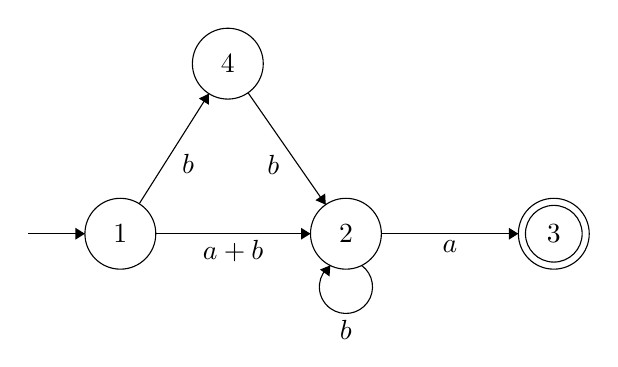
\begin{tikzpicture}[scale=0.15]
            \tikzstyle{every node}+=[inner sep=0pt]
            \draw [black] (17.6,-26.1) circle (3);
            \draw (17.6,-26.1) node {$1$};
            \draw [black] (36.7,-26.1) circle (3);
            \draw (36.7,-26.1) node {$2$};
            \draw [black] (26.7,-11.7) circle (3);
            \draw (26.7,-11.7) node {$4$};
            \draw [black] (54.3,-26.1) circle (3);
            \draw (54.3,-26.1) node {$3$};
            \draw [black] (54.3,-26.1) circle (2.4);
            \draw [black] (9.8,-26.1) -- (14.6,-26.1);
            \fill [black] (14.6,-26.1) -- (13.8,-25.6) -- (13.8,-26.6);
            \draw [black] (19.2,-23.56) -- (25.1,-14.24);
            \fill [black] (25.1,-14.24) -- (24.25,-14.65) -- (25.09,-15.18);
            \draw (22.78,-20.2) node [right] {$b$};
            \draw [black] (28.41,-14.16) -- (34.99,-23.64);
            \fill [black] (34.99,-23.64) -- (34.94,-22.69) -- (34.12,-23.26);
            \draw (31.1,-20.26) node [left] {$b$};
            \draw [black] (20.6,-26.1) -- (33.7,-26.1);
            \fill [black] (33.7,-26.1) -- (32.9,-25.6) -- (32.9,-26.6);
            \draw (27.15,-26.6) node [below] {$a+b$};
            \draw [black] (38.023,-28.78) arc (54:-234:2.25);
            \draw (36.7,-33.35) node [below] {$b$};
            \fill [black] (35.38,-28.78) -- (34.5,-29.13) -- (35.31,-29.72);
            \draw [black] (39.7,-26.1) -- (51.3,-26.1);
            \fill [black] (51.3,-26.1) -- (50.5,-25.6) -- (50.5,-26.6);
            \draw (45.5,-26.6) node [below] {$a$};
        \end{tikzpicture}
    \end{center}
    Observe in what way 2 acts as an intermediate state.
    \begin{itemize}
        \item From 1 to 3: $(a+b){b^*}a$
        \item From 4 to 3: $b{b^*}a$
    \end{itemize}
\end{frame}

\begin{frame}{Example}
    Remove state 2 and its associated edges. Add to edges 1 to 3 and 4 to 3 the intermediate regular expressions.
    \begin{center}
        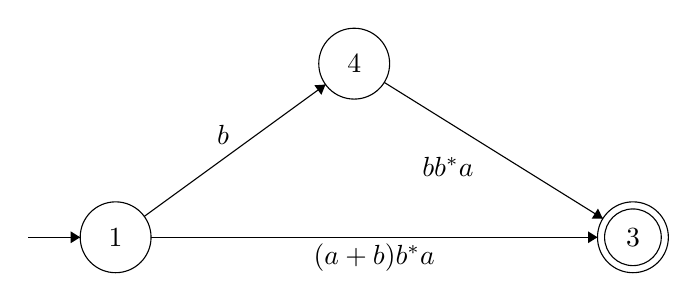
\begin{tikzpicture}[scale=0.15]
            \tikzstyle{every node}+=[inner sep=0pt]
            \draw [black] (10.6,-29.5) circle (3);
            \draw (10.6,-29.5) node {$1$};
            \draw [black] (54.4,-29.5) circle (3);
            \draw (54.4,-29.5) node {$3$};
            \draw [black] (54.4,-29.5) circle (2.4);
            \draw [black] (30.8,-14.8) circle (3);
            \draw (30.8,-14.8) node {$4$};
            \draw [black] (3.2,-29.5) -- (7.6,-29.5);
            \fill [black] (7.6,-29.5) -- (6.8,-29) -- (6.8,-30);
            \draw [black] (13.03,-27.73) -- (28.37,-16.57);
            \fill [black] (28.37,-16.57) -- (27.43,-16.63) -- (28.02,-17.44);
            \draw (19.7,-21.65) node [above] {$b$};
            \draw [black] (13.6,-29.5) -- (51.4,-29.5);
            \fill [black] (51.4,-29.5) -- (50.6,-29) -- (50.6,-30);
            \draw (32.5,-30) node [below] {$(a+b){b^*}a$};
            \draw [black] (33.35,-16.39) -- (51.85,-27.91);
            \fill [black] (51.85,-27.91) -- (51.44,-27.07) -- (50.91,-27.92);
            \draw (38.73,-22.65) node [below] {$b{b^*}a$};
        \end{tikzpicture}
    \end{center}
\end{frame}

\begin{frame}{Example}
    Pick state 4 to remove and find how it acts as an intermediate state.
    \begin{itemize}
        \item From 1 to 3: $(a+b){b^*}a+bb{b^*}a$
    \end{itemize}
    Remove state 4 and its associated edges. Add to edges 1 to 3 the intermediate regular expression.
    \begin{center}
        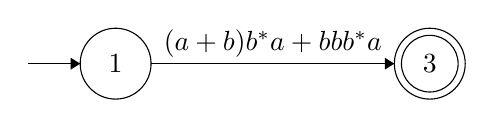
\begin{tikzpicture}[scale=0.15]
            \tikzstyle{every node}+=[inner sep=0pt]
            \draw [black] (8.2,-28.5) circle (3);
            \draw (8.2,-28.5) node {$1$};
            \draw [black] (34.8,-28.5) circle (3);
            \draw (34.8,-28.5) node {$3$};
            \draw [black] (34.8,-28.5) circle (2.4);
            \draw [black] (0.8,-28.5) -- (5.2,-28.5);
            \fill [black] (5.2,-28.5) -- (4.4,-28) -- (4.4,-29);
            \draw [black] (11.2,-28.5) -- (31.8,-28.5);
            \fill [black] (31.8,-28.5) -- (31,-28) -- (31,-29);
            \draw (21.5,-28) node [above] {$(a+b){b^*}a+bb{b^*}a$};
        \end{tikzpicture}
    \end{center}
    Obtain the final regular expression: $(a+b){b^*}a+bb{b^*}a$
\end{frame}

\begin{frame}[t]{Exercise}
    \textbf{Exercise.} Find a regular expression that denotes the language $L = \{w \in \{0,1\}^* : n_0(w) \mod 2 = 0 \And n_1(w) \mod 2 = 0\}$
\end{frame}

\begin{frame}{Regular expressions and regular languages}
    \textbf{Theorem.} The family of languages accepted by regular expressions is exactly the same as the family of languages accepted by FAs. Or, in other words, a language $L$ is regular if and only if there exists a regular expression $r$ such that $L = L(r)$.
\end{frame}

\end{document}
